\documentclass{article}
\usepackage[version=4]{mhchem}
\usepackage{siunitx}
\usepackage{fancyhdr}
\usepackage{graphicx}
\graphicspath{ {images/}}
\pagestyle{fancy}

\author{J.R. Powers-Luhn}
\date{2016/01/25}
\title{Chemistry 580 Notes}

\rhead{J.R. Powers-Luhn}

\begin{document}

\section{Atomic Structure}

\subsection{Atoms}

\subsubsection{Elements and atoms}
Isobar means nuclides with the same mass number A but with a different number of protons and neutrons. Isotone means nuclides with the same number of neutrons but different numbers of protons. (Shultis, 10)

\subsubsection{Atomic structure}
The notes cite an electron radius of \SI{1e-15}{\meter} while Shultis cites a radius of \SI{1e-19}{\meter} (Shultis, 7). Modern Physics, however, treats the electron as a point charge without radius (Curtis, 74).

\subsubsection{Problems}
Look up the atomic numbers (Z) of:
\begin{itemize}
    \item Sr: 38
    \item Cu: 29
    \item Ag: 47
    \item Os: 76
\end{itemize}
Draw the structures of the three isotopes
\begin{itemize}
    \item \ce{^{64}Zn} \\
$\left[30 \mathrm{p}^+ \right]$  $30 \mathrm{e}^-$ \\
$\left[34 \mathrm{n} \right]$ 
    \item \ce{^{65}Zn} \\
$\left[30 \mathrm{p}^+ \right]$  $30 \mathrm{e}^-$ \\
$\left[35 \mathrm{n} \right]$ 
    \item \ce{^{66}Zn} \\
$\left[30 \mathrm{p}^+ \right]$  $30 \mathrm{e}^-$ \\
$\left[36 \mathrm{n} \right]$ 
\end{itemize}
Write designations for the three isotopes in Problem 1.03b
\begin{itemize}
    \item{\ce{^{64}_{30}Zn}}
    \item{\ce{^{65}_{30}Zn}}
    \item{\ce{^{66}_{30}Zn}}
\end{itemize}
Draw complete structures and give full symbols for:
\begin{itemize}
    \item \ce{^{26}Al} \vspace{10mm}
    \item \ce{^{94}Mo} \vspace{10mm}
    \item \ce{^{159}Tb} \vspace{10mm}
\end{itemize}

\subsubsection{Atomic (nuclidic) properties}
Even though the liquid drop model ignores the nature of neutrons and protons it is still very good at predicting decay modes and susceptability to fission (Shultis, 68)

\subsubsection{Atom types}
Atom comes from the Greek word meaning "indivisible". Wrong!

\subsubsection{Problems}
Indicate the nuclear charge in:
\begin{itemize}
    \item \ce{Mn}: 25+
    \item \ce{Np}: 93+
\end{itemize}
Calculate the nuclear radius of:
\begin{itemize}
    \item \ce{^{102}Ru}: \SI{6.54e-13}{\centi\meter}
\end{itemize}
Calculate the nuclear mass of:
\begin{itemize}
    \item \ce{^{22}Ne}: 21.9793 amu
\end{itemize}
Look up the mass in me of \ce{^{21}Ne}. Then add the masses of the constituent particles. Explain the discrepancy.
\begin{itemize}
    \item Mass of \ce{^{21}Ne}: \SI{20.99384668}{\amu}
    \item Mass of constituents: $11 m_n + 10 m_p + 10 m_e = \SI{21.1736}{\amu} $.
    \item The difference is in the binding energy of the \ce{^{21}Ne} nucleus.
\end{itemize}
Calculate the binding energy per nucleon for \ce{^{50}Ti}
$$ \frac{\left(28 m_n + 22 m_p + 22 m_e - m_{Ti-50} \right) c^2 }{50} = \SI{8.75757}{\mega\electronvolt} $$
Draw three isotopes with a Z=25:
\begin{itemize}
    \item{\ce{^{53}_{25}Mn}}
    \item{\ce{^{54}_{25}Mn}}
    \item{\ce{^{52}_{25}Mn}}
\end{itemize}
Draw three isotones with a N=51
\begin{itemize}
    \item{\ce{^{51}_{25}Mn}}
    \item{\ce{^{52}_{26}Fe}}
    \item{\ce{^{50}_{24}Cr}}
\end{itemize}
Draw three isobars with an A=40
\begin{itemize}
    \item{\ce{^{40}_{20}Ca}}
    \item{\ce{^{40}_{21}Sc}}
    \item{\ce{^{40}_{19}K}}
\end{itemize}
Identify the nuclide with an:
\begin{itemize}
    \item I=0: {\ce{^{64}_{30}Zn}}
    \item I=0: {\ce{^{46}_{34}Se}}
    \item I=n/2: {\ce{^{25}_{12}Mg}}
\end{itemize}

\subsubsection{Occurrences}
The shell model of the nucleus has been very successful in predicting the total angular momentum of the nucleus, the transitions of metastable states, and the characteristic of beta and gamma decay, as well as the magnetic moment of the nuclei. It parallels the quantum mechanical solution of the electrons orbiting the nucleus but must make assumptions about the quantized angular momentum of the nucleons (Shultis, 70).

\subsubsection{Even and odd generalizations}
Nitrogen-14 is weird. Why is it stable? This makes no sense. Apparently the bound proton is slightly less massive than the bound neutron in Oxygen-14, meaning Nitrogen-14 has a higher binding energy per nucleon, but it still makes no sense (citation needed). 

\subsubsection{Magic numbers (nuclear shells)}
Even numbers of protons or neutrons are favored because these particles are fermions (spin of n/2 (Shultis, 7)). Fermions can only have one particle at a given combination of quantum numbers (energy, spin, angular momentum), while bosons can have any number of particles (their wave equations do not interfere destructively).

\subsubsection{Stable-atom systematics}
Nuclides above Z=83 are unstable, but spontaneous fission does not begin until Z=92 (Uranium-233). Even then it has a very low chance of occurring at \num{1.3e-10}\% (Shultis, 141).

\subsubsection{Problems}
Calculate the average atomic weight of the element when \ce{Br} has 50.54\% \ce{^{79}Br} and 49.46\% \ce{^{81}Br}
$$ 0.5054 m_{Br-79} + 0.4946 m_{Br-81} = \SI{79.9065}{\amu}
$$
Identify an element which has 7 stable isotopes: \textbf{Ruthenium}

Identify an element which shows either a magic neutron number only or a magic proton number only. What sign of extra stability do you find in it? \textbf{\ce{^3He} is stable with an odd number of neutrons. Since it is so small, the nuclear strong force is still applicable to all nucleons, meaning that they are all tightly bound.}

Plot a graph of the average atomic weight of the elements up through Th minus the atomic number against the atomic number. How is this line related to the stability band?
\begin{figure}[h]
    \centering
    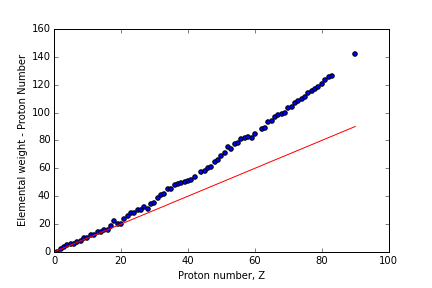
\includegraphics[width=10cm,height=5cm,keepaspectratio]{stability_line}
    \caption{Element weight minus number vs element number}
    \label{fig:stability_line}
\end{figure}
\textbf{This plotted points in figure \ref{fig:stability_line} are the center of the stability line.}


\newpage

\section{Radioactivity}

\subsection{Radioatoms or Radionuclides}

\subsubsection{Types of instability}
Typical $\alpha$ particle emission energies are $<\SI{10}{\mega\electronvolt}$, meaning that relativistic effects can be ignored. The decay energy is expressed by (Shultis, 95): $$ E_D = Q_\alpha \left[ \frac{M_\alpha}{M_D + M_\alpha} \right] \approx Q_\alpha \left[\frac{A_\alpha}{A_D + A_\alpha} \right] $$

\subsubsection{Neutron-rich radionuclides}
Because there are three particles emitted in $ \beta^- $ decay (daughter nucleus, electron, and electron-antineutrino), there is no unique solution to the energies of the resultant particles. The results are bound at the high end by the antineutrino having zero kinetic energy (Shultis, 97).

\newpage

\subsubsection{Neutron-deficient radionuclides}
Generally the process of electron capture leaves the nucleus in an excited state, implying that a gamma must be emmitted sometime later (Shultis, 89).

\newpage

\subsubsection{Other decay types}
Unlike $\beta$ decay, $\alpha$ decay has only two products (daughter nucleus and $\alpha$ particle), so conservation of momentum can be used to solve for the kinetic energy of the daughter nucleus and $\alpha$ (Shultis, 95).

\subsubsection{Problems}
Write complete equations for the beta decay of \ce{^{105}Ru} and \ce{^{142}Ba}
\begin{itemize}
    \item \ce{^{105}_{44}Ru^0 \rightarrow ^{105}_{45}Rh^+ + ^0_{-1}\beta^- + ^0_0\nu^0}
    \item \ce{^{142}_{56}Ba^0 \rightarrow ^{142}_{57}La^+ + ^0_{-1}\beta^- + ^0_0\nu^0}
\end{itemize}
Write complete equations for the beta decay of \ce{^{61}Zn} and \ce{^{111}Sn}
\begin{itemize}
    \item \ce{^{61}_{30}Zn^0 \rightarrow ^{61}_{29}Cu^- + ^0_{-1}\beta^+ + ^0_0\nu^0}
    \item \ce{^{111}_{50}Sn^0 \rightarrow ^{111}_{49}In^- + ^0_{-1}\beta^+ + ^0_0\nu^0}
\end{itemize}
Write complete equations for the electron capture decay of \ce{^{134}Cs} and \ce{^{172}Ta}
\begin{itemize}
    \item \ce{^{134}_{55}Cs^+ + ^0_{-1}e^- \rightarrow ^{134}_{54}Cu^0 + ^0_0\nu^0}
    \item \ce{^{172}_{73}Ta^+ + ^0_{-1}e^- \rightarrow ^{172}_{72}In^0 + ^0_0\nu^0}
\end{itemize}
Write complete equations for the alpha decay of \ce{^{210}Ru} and \ce{^{250}Cf}
\begin{itemize}
    \item \ce{^{210}_{44}Ru^0 \rightarrow ^{206}_{42}Mo^{-2} + ^4_2\nu^{+2}}
    \item \ce{^{250}_{98}Cf^0 \rightarrow ^{246}_{96}Cm^{-2} + ^4_2\nu^{+2}}
\end{itemize}
Write a complete equation for the gamma decay of \ce{^{69m}Zn}
\begin{itemize}
    \item \ce{^{69m}_{44}Ru^0 \rightarrow ^{206}_{42}Mo^{-2} + ^4_2\nu^{+2}}
\end{itemize}

\subsubsection{Predicting decay}
The liquid drop model with appropriate corrections gives a line of stability calculation of:
\begin{equation}
    Z(A) = \left( \frac{A}{2} \right) \frac{1+\left(m_n-m_p\right)c^2 / \left(4 a_a \right)}{1 + a_cA^{2/3} / \left(4 a_a \right)}
\end{equation}
Above this line, the nuclide will emit $\beta^+$, below it it will emit $\beta^-$ (Shultis, 69).

\subsubsection{Problems}
Predict the probable decay of:
\begin{itemize}
    \item \ce{^{67}Cu}: $\beta^-$ (correct)
    \item \ce{^{64}Cu}: Stable (beta+ or beta-)
    \item \ce{^{112}In}: $beta^+$ (beta+ or beta-)
    \item \ce{^{115}Cd}: $beta^-$ (correct)
    \item \ce{^{232}Th}: $\alpha$ (or SF)
    \item \ce{^{248}Es}: $\alpha$ (or beta+)
\end{itemize}

\newpage

\subsubsection{Mass-energy relationships}


\end{document}
